% Syllabus Template from Arman Shokrollahi
% https://www.overleaf.com/latex/templates/syllabus-template-course-info/gbqbpcdgvxjs

\documentclass[11pt, letterpaper]{article}
%\usepackage{geometry}
\usepackage[inner=2cm,outer=2cm,top=2.5cm,bottom=2.5cm]{geometry}
\pagestyle{empty}
\usepackage{graphicx}
\usepackage{fancyhdr, lastpage, bbding, pmboxdraw}
\usepackage[usenames,dvipsnames]{color}
\definecolor{darkblue}{rgb}{0,0,.6}
\definecolor{darkred}{rgb}{.7,0,0}
\definecolor{darkgreen}{rgb}{0,.6,0}
\definecolor{red}{rgb}{.98,0,0}
\usepackage[colorlinks,pagebackref,pdfusetitle,urlcolor=darkblue,citecolor=darkblue,linkcolor=darkred,bookmarksnumbered,plainpages=false]{hyperref}
\renewcommand{\thefootnote}{\fnsymbol{footnote}}

\pagestyle{fancyplain}
\fancyhf{}
\lhead{ \fancyplain{}{The Science of Cities} }
%\chead{ \fancyplain{}{} }
\rhead{ \fancyplain{}{Spring 2022} }%\today
%\rfoot{\fancyplain{}{page \thepage\ of \pageref{LastPage}}}
\fancyfoot[RO, LE] {page \thepage\ of \pageref{LastPage} }
\thispagestyle{plain}

%%%%%%%%%%%% LISTING %%%
\usepackage{listings}
\usepackage{caption}
\usepackage{setspace}
\DeclareCaptionFont{white}{\color{white}}
\DeclareCaptionFormat{listing}{\colorbox{gray}{\parbox{\textwidth}{#1#2#3}}}
\captionsetup[lstlisting]{format=listing,labelfont=white,textfont=white}
\usepackage{verbatim} % used to display code
\usepackage{fancyvrb}
\usepackage{acronym}
\usepackage{amsthm}
\VerbatimFootnotes % Required, otherwise verbatim does not work in footnotes!



\definecolor{OliveGreen}{cmyk}{0.64,0,0.95,0.40}
\definecolor{CadetBlue}{cmyk}{0.62,0.57,0.23,0}
\definecolor{lightlightgray}{gray}{0.93}



\lstset{
%language=bash,                          % Code langugage
basicstyle=\ttfamily,                   % Code font, Examples: \footnotesize, \ttfamily
keywordstyle=\color{OliveGreen},        % Keywords font ('*' = uppercase)
commentstyle=\color{gray},              % Comments font
numbers=left,                           % Line nums position
numberstyle=\tiny,                      % Line-numbers fonts
stepnumber=1,                           % Step between two line-numbers
numbersep=5pt,                          % How far are line-numbers from code
backgroundcolor=\color{lightlightgray}, % Choose background color
frame=none,                             % A frame around the code
tabsize=2,                              % Default tab size
captionpos=t,                           % Caption-position = bottom
breaklines=true,                        % Automatic line breaking?
breakatwhitespace=false,                % Automatic breaks only at whitespace?
showspaces=false,                       % Dont make spaces visible
showtabs=false,                         % Dont make tabls visible
columns=flexible,                       % Column format
morekeywords={__global__, __device__},  % CUDA specific keywords
}

%%%%%%%%%%%%%%%%%%%%%%%%%%%%%%%%%%%%
\begin{document}
\begin{center}
{\Large \textsc{POLS 4641: The Science of Cities}}
\end{center}
\begin{center}
{\large Spring 2022}
\end{center}

\begin{center}
\rule{6.5in}{0.4pt}
\begin{minipage}[t]{.96\textwidth}
\begin{tabular}{llcccll}
\textbf{Professor:} & Joe Ornstein & & &  & \textbf{Time:} & TTh 9:35am -- 10:50pm \\
\textbf{Email:} &  \href{mailto:jornstein@uga.edu}{jornstein@uga.edu} & & & & \textbf{Place:} & 101D Baldwin Hall\\
\textbf{Website:} & \href{https://joeornstein.github.io/pols-4641/}{https://joeornstein.github.io/pols-4641/} & & & & &
\end{tabular}
\end{minipage}
\rule{6.5in}{0.4pt}
\end{center}
\vspace{.15cm}
\setlength{\unitlength}{1in}
\renewcommand{\arraystretch}{2}

\begin{figure}[h]
	\centering
	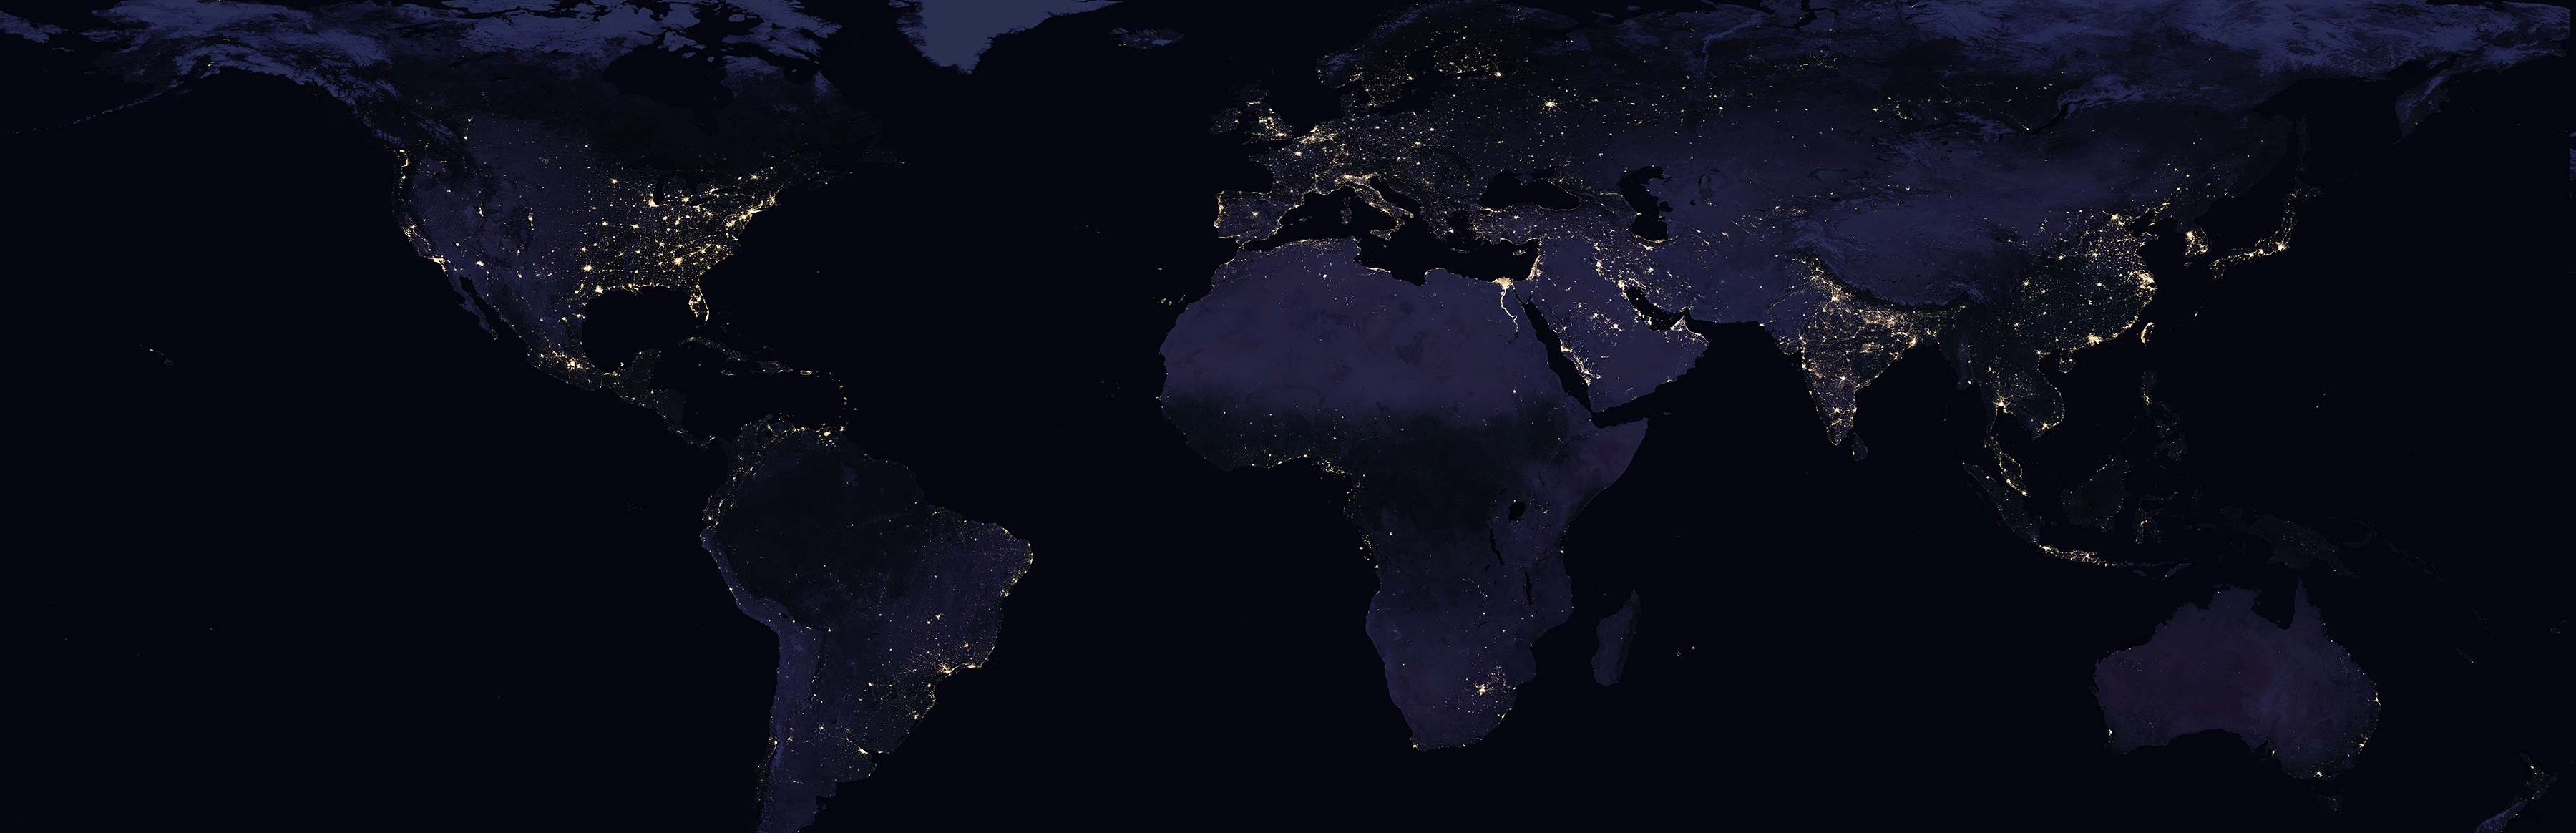
\includegraphics[width = 1.03\textwidth]{img/night-lights-cropped.jpg}
\end{figure}

%\begin{quotation}
%	\noindent``\textit{You can't really know anything if you just remember isolated facts. If the facts don't hang together on a latticework of theory, you don't have them in a usable form. You've got to have models in your head.}''\\
%	\\
%	--Charlie Munger (investor, vice chairman of Berkshire Hathaway)
%\end{quotation}

%% PREAMBLE %%
\onehalfspacing

% Loosely guessed from this: https://www.sciencealert.com/half-the-world-s-population-lives-on-1-of-its-land

\noindent Over half of the Earth's population lives within the sea of city lights visible on the satellite map above. These cities are the centers of global commerce and culture, but in order to function, they require effective governance. Cities need roads, schools, police, fire protection, parks, buses, sewers, and electricity. Many of our most pressing political problems --- including education, criminal justice reform, housing, and climate change --- are in large part problems of city politics.

In this course, we will explore what makes cities tick, and how research from political science, economics, sociology, psychology, and mathematics can help us build cities that are healthier, safer, fairer, and more livable for their residents. We'll begin with foundational research on the origins of cities and how best to govern them, then discuss some of the specific policy challenges faced by cities today, and end the semester with a few questions about the future of cities, both in the US and worldwide.

%\section*{Course Objectives}
%%\vskip.15in
%%\noindent\textbf{Course Objectives:}  
%By the end of this course, you will be able to:
%\begin{itemize}
%	\item 
%	\item 
%	\item
%\end{itemize}


\section*{Course Structure}

The class will meet twice a week, and each class period will be devoted to a particular topic. You can find the complete list of topics and schedule on the \href{https://joeornstein.github.io/pols-4641/}{class website}. At the beginning of the semester, we will split the class into teams of five or six students. Every day, one member from each team will be responsible for researching that days' topic and writing a paper that serves as a \textbf{Table Read} for the class session. Class time will be structured like a  \href{https://medium.com/swlh/the-silent-meeting-manifesto-v1-189e9e3487eb}{Silent Meeting}, where we take time to read our fellow students' papers and offer comments and suggestions. These comments will both motivate class discussion and help the students revise their papers for final submission. Our agenda for most class days will look like this:

\begin{enumerate}
\item Introduction (5 minutes)
\item Table Read (15 minutes)
\item Team Discussion and Revisions (20 minutes)
\item Class Discussion (20 minutes)
\item Closing Thoughts (5 minutes)
\end{enumerate}

Each student will write five papers over the course of the semester, and teams can divide the topics among themselves however they choose. Papers should be roughly 2000-3000 words (about 6 pages), short enough to read in 10-15 minutes. After your table read, you have 24 hours to make any revisions and submit the paper. Late papers will be marked down a full letter grade per 24 hours.
 
Why structure the course this way? Well, originally it was an on-the-fly adjustment to remote learning during the COVID-19 pandemic. But the structure proved popular and enduring, because it offers a few nice benefits:

\begin{itemize}
	\item It sure beats sitting for an hour and getting talked at.
	\item Your papers don't just get skimmed by your professor and discarded; they're the primary way your peers will learn about the material that day, which makes writing a paper for class less pointless.
	\item Everyone gets peer feedback on their work and a chance to improve.
	\item Everyone can contribute during class, regardless of background knowledge or comfort with public speaking. (I, for example, tend to get nervous when asked to speak in front of 45 of my peers, but I’m happy making comments on a Google Doc. Perhaps you are like me.)
	\item The class project isn't something that gets tacked on at the end of the semester. Researching and writing your papers will be your primary intellectual activity during the course.
\end{itemize}

\noindent During the Table Read portion of class, take time to first read the paper from beginning to end, then go back and add comments, questions, and suggestions for edits in the margins of the shared document. Don't worry that criticism will harm your peers' grades! Quite the opposite. If you frame your critiques as suggestions, it can only help them improve the draft and get a better grade upon final submission (due 24 hours after the Table Read). Your comments can take any form: grammatical edits, suggestions for how to make a point more clearly, clarification questions, flags for further discussion, and points of agreement/disagreement. And don't forget: positive feedback is just as important as negative feedback! If you read something that was thought-provoking or interesting, highlight it!

Once the silent portion of class is over, we will have a more traditional ``loud'' discussion, focusing on deeper questions brought up during the Table Read.

\section*{COVID-19 Precautions}

Due to the COVID-19 pandemic, I expect that there will be more than the usual share of setbacks and hardships this semester. Please don't hesitate to ask questions or reach out to me with your concerns. If you test positive for COVID-19, please isolate for five days and report the positive test through \href{https://dawgcheck.uga.edu/}{DawgCheck} (woof woof), which will automatically inform me that you'll be missing class for a few days. Given the structure of the course, you can easily miss a couple of classes and catch up by reading the Table Reads. See \href{https://ovpi.uga.edu/_resources/documents/Syllabi-Info-for-Students-Spring-2022.pdf}{this page} for more up-to-date and detailed guidance.

\section*{Grading}

During the semester, I will select three of your papers at random to grade, and your final grade will be the average of those three paper grades. I have high standards for the papers you submit, because your classmates will be relying on your paper to help understand the topic that day. In other classes, bad papers might be painful for the professors who read them, but they don't actually \textit{harm} anyone. In this class, they do! So I expect your effort to be commensurate with that responsibility. I grade papers on a 4-point (GPA) scale using the following four-part rubric:

\subsection*{Accurate}

\begin{itemize}
	\item \textbf{1 point:} The paper either fails to engage with the scientific research on the topic, or does so in a mostly misleading way.
	\item \textbf{2 points:} There are one or more major mistakes that mislead the reader about the scientific research on the topic.
	\item \textbf{3 points}: There may be few minor inaccuracies, but nothing terribly misleading.
	\item \textbf{4 points:} The paper accurately portrays the scientific research, including some of the denser pieces you were assigned to read. Impressively done!
\end{itemize}

\subsection*{Clear}

\begin{itemize}
	\item \textbf{1 point:} The paper lacks a clear organization, and I have trouble understanding its meaning.
	\item \textbf{2 points:} While reading your paper, I often had trouble understanding your point or following your train of thought.
	\item \textbf{3 points:} The paper was clear, but there were a few places where I had trouble understanding your point or following your train of thought.
	\item \textbf{4 points:} This is a paper of exceptional clarity. I understood everything you were trying to say, and the paper was well-organized so that I could easily follow your train of thought.
\end{itemize}

\subsection*{Meticulous}

\begin{itemize}
	\item \textbf{1 point:} The paper contains relatively few ideas and only cites a few sources.
	\item \textbf{2 points:} There are several good ideas in here, but there are a lot more facts/ideas/arguments you could have packed into 2000-3000 words.
	\item \textbf{3 points:} This is a well-researched and thoughtful paper, although there are a few places where I wish you would have added more detail.
	\item \textbf{4 points:} The paper is brimming with facts and ideas from a large array of sources, thoughtfully woven together into a coherent thesis.
\end{itemize}


\subsection*{Entertaining}

\begin{itemize}
	\item \textbf{1 point:} The paper was difficult to read. 
	\item \textbf{2 points:} The paper has some entertaining parts, but it is mostly difficult to read.
	\item \textbf{3 points:} This paper was fun to read, but dry in a few places. It could use some ``punching up''.
	\item \textbf{4 points:} This paper was really fun to read! In several places, it may have elicited a physical emotional response -- like laughter, tears, or spontaneous dancing.
\end{itemize}




\section*{Office Hours}

I will be available for office hours by appointment, and you can sign up for 15 minute slots through the course website. With each paper draft, you'll simultaneously be learning new content \textit{and} trying to teach others what you've learned. This is a difficult task! I strongly recommend that you sign up for office hours before your table read is due so we can discuss any questions you have about the material you're reading. Even if you don't have a problem with the material, stop by office hours anyway! One of the great things about college is that your professors are all required to set aside time each week just to talk with their students. And, not to brag, but I'm \textit{pretty good at talking}. My job title (Assistant Professor) is basically just Latin for ``Assistant Talker''.

%\section*{Course Topics}
%
%Ultimately, the content that we cover will depend on what questions you decide to write about. Below is a list of suggested paper topics, and I will provide a set of readings for each topic on the course \href{https://uga.view.usg.edu/d2l/home/2213495}{eLC page}. Take a few minutes to read over the prompts below and decide which you would most like to address in your paper. Then send me an email introducing yourself and ranking your top 10 choices. (If you'd like to suggest your own topic, please do! We'll work together to compile a good reading list.) Once I've assigned everyone's topics, I will post a schedule for the semester.
%
%\textbf{Note:} I will write the Table Reads for the first two weeks of class, so no one is given too tight a deadline, and so you get a chance to read some examples of the kind of papers that I expect.
%
%%\subsection*{Week 1: Course Introduction}
%%
%%\begin{itemize}
%%	\item How will the course be organized? What do you need to be successful?
%%	\item What makes for a good essay?
%%\end{itemize}
%%
%%\subsection*{Week 2: Why Cities?}
%%
%%\begin{itemize}
%%	\item MLK Day
%%	\item Why cities? %plus monocentric city model
%%	\item Why are some cities in strange places?
%%\end{itemize}
%
%\subsection*{Historical Questions}
%
%\begin{itemize}
%	\item When and where were the very first city-states established? What enabled these cities to form, and what made them so fragile and prone to collapse? % against the grain / scott alexander...jared diamond?
%	\item Where did urbanization occur prior to the Industrial Revolution and why?
%	\item What does urbanization do to us, culturally \& psychologically?
%\end{itemize}
%	
%
%\subsection*{The Urban-Rural Divide}
%
%\begin{itemize}
%	\item What caused the geographic divide between liberals and conservatives? % the big sort
%	\item Why are the interests of city residents underrepresented in national government? % Why are they underrespresented in national government. Why do cities lose?
%	%\item Many US cities are overwhelmingly represented by Democratic lawmakers. Is such single-party dominance harmful?
%	\item Does it matter whether Democrats or Republicans are in charge of city government?
%\end{itemize}
%
%\subsection*{Federalism}
%
%\begin{itemize}
%	\item The Atlanta metropolitan area contains roughly 140 municipal governments. What are the benefits (and drawbacks) of dividing a city this way?
%	\item What are the benefits (and drawbacks) of dividing the \textit{responsibilities} of governing across multiple overlapping governments (e.g. municipalities, school boards, special districts)? % TODO John Oliver, Christopher Berry
%	\item During the late 20th century, many city governments fell deeply into debt and/or bankruptcy. What causes cities to lose money? Are we likely to see more municipal bankruptcies in the next decade?
%\end{itemize}
%
%\subsection*{City Limits}
%
%\begin{itemize}
%	\item Why don't liberal cities enact their own social welfare programs? % City limits
%	\item Do economic development incentives (i.e. ``corporate welfare'') produce value, or do they just produce a ``race to the bottom''?
%	\item Should local governments be spending so much money on sports stadiums?
%	\item How well do city governments represent their citizens?
%\end{itemize}
%
%\subsection*{Crime \& Policing}
%
%\begin{itemize}
%	\item What caused the spike in violent crime from 1970 to 1990 and its subsequent decline?
%	%\item Are we facing a new wave in crime in major US cities? Why or why not?
%	\item What reforms work best to reduce police violence?
%\end{itemize}
%
%\subsection*{Public Health}
%
%\begin{itemize}
%	\item Did urban density exacerbate the spread of COVID-19?
%	\item What are the most effective things that cities have done to promote public health? %TODO Walkability stuff, John Snow, smoking ban literature, built environment, etc.
%\end{itemize}
%
%\subsection*{Race \& Segregation}
%
%\begin{itemize}
%	\item Why is residential segregation such a persistent problem in US cities?
%	\item What are the long-run effects of residential segregation? %TODO Ryan Enos racial threat stuff, Trounstine
%	%\item What was the Great Migration, and what were its long-term effects?
%\end{itemize}
%
%\subsection*{Corruption}
%
%\begin{itemize}
%	\item What works to curb corruption in city government?
%	\item What was ``machine politics'', and where did it go?
%\end{itemize}
%
%\subsection*{Political Institutions}
%
%\begin{itemize}
%	\item Do municipal political institutions matter? For instance, does it matter whether your city is run by a mayor or a manager? Does it matter whether your city council is elected at-large? Do ballot initiatives and popular referenda improve governance, or make it more chaotic?
%	\item Does it matter \textit{when} cities hold their elections?
%	\item How has the decline of local news media affected local politics?
%\end{itemize}
%
%
%
%\subsection*{Transportation}
%
%\begin{itemize}
%	\item What were the long-term effects of the Interstate Highway System on US cities?
%	\item Why do American cities sprawl while European cities are compact? And how does it affect our quality of life?
%	\item What makes a city walkable? Bikable? What are the most cost effective ways to improve multi-modal transit? %TODO transit-oriented development
%	\item Why are mass transit projects so expensive in the United States compared to peer nations?
%	\item Do US cities have too few or too many parking spaces? Why?
%	\item What steps can city governments take to mitigate climate change? %TODO triumph of the cities passages
%\end{itemize}
%
%\subsection*{Housing}
%
%\begin{itemize}
%	\item Why have home prices gotten so expensive in major cities?
%	\item Why is it so hard to build more housing where we need it? 
%	\item What works to reduce homelessness? %(Housing First papers, etc.)
%	\item How common are residential evictions, who do they most burden, and what are some effective remedies? %TODO Evicted book
%	% \item Something something public housing
%\end{itemize}
%
%\subsection*{Urban Decline in Industrialized Nations}
%
%\begin{itemize}
%	\item Where are Americans moving and what explains these migration patterns?
%	\item Where have cities shrunk from their population peak? What makes urban decline so difficult to manage?
%	\item Why do so many well-meaning (and not-so-well-meaning) Urban Renewal plans fail? % Seeing like a state, (Belmermeir podcast) High-modernism and its failings.  
%	%TODO This one is pretty broad. We could split it into two. Triumph of the city boondoggles chapter in one; high modernism in another.
%	%\item How severe is the ``infrastructure deficit'' in American cities? Why do governments often underinvest in critical infrastructure? % Flint, smart cities
%	\item Will the ``Death of Distance'' hurt or help cities in the long run?
%\end{itemize}
%
%\subsection*{Urbanization in the Developing World}
%
%\begin{itemize}
%	\item What explains the tremendous growth of ``primate cities'' (Mexico City, Bangkok, Jakarta, Lagos, Kinshasa, etc.)?
%	\item Is urbanization helpful or harmful for the poor in developing countries? % Glaser
%	\item What programs and policies can best help those living in urban slums?
%	\item How has China achieved such rapid urbanization? What are the effects of this massive internal migration on Chinese society? % the Chinese Mayor, dual sector model, Lewis point
%\end{itemize}



%\end{flushleft}
%\end{minipage}
%\end{center}

%\vskip.15in
%\noindent\textbf{Important Dates:}
%\begin{center} \begin{minipage}{3.8in}
%\begin{flushleft}
%Midterm \#1      \dotfill ~\={A}b\={a}n 16, 1393  \\
%Midterm \#2      \dotfill ~\={A}zar 21, 1393  \\
%%Project Deadline \dotfill ~Month Day \\
%Final Exam       \dotfill ~Dey 18, 1393  \\
%\end{flushleft}
%\end{minipage}
%\end{center}



\section*{Academic Honesty}

Remember that when you joined the University of Georgia community, you agreed to abide by a code of conduct outlined in the academic honesty policy called \href{https://honesty.uga.edu/Academic-Honesty-Policy/Introduction/}{\textit{A Culture of Honesty}}. It has some pretty specific things to say on the subject of cheating. Quite specific. Plagiarized papers are unacceptable, and I will report any and all dishonest conduct to the Office of the Vice President for Instruction.

\section*{Mental Health and Wellness Resources}

\begin{itemize}
\item If you or someone you know needs assistance, you are encouraged to contact Student Care and Outreach in the Division of Student Affairs at 706-542-7774 or visit \href{https://sco.uga.edu}{https://sco.uga.edu}. They will help you navigate any difficult circumstances you may be facing by connecting you with the appropriate resources or services. 
\item UGA has several resources for a student seeking \href{https://www.uhs.uga.edu/bewelluga/bewelluga}{mental health services} or \href{https://www.uhs.uga.edu/info/emergencies}{crisis support}. 
\item If you need help managing stress anxiety, relationships, etc., please visit \href{https://www.uhs.uga.edu/bewelluga/bewelluga}{BeWellUGA} for a list of FREE workshops, classes, mentoring, and health coaching led by licensed clinicians and health educators in the University Health Center.
\item Additional resources can be accessed through the UGA App.
\end{itemize}



%%%%%% THE END 
\end{document} 